\documentclass[sigplan, screen]{acmart}

%\settopmatter{printfolios=true,printccs=false,printacmref=false}
%\settopmatter{printfolios=false,printccs=false,printacmref=false}
\usepackage{graphicx}
\usepackage{listings}
\usepackage{enumitem}

% URL PACKAGE HACK
\expandafter\def\expandafter\UrlBreaks\expandafter{\UrlBreaks%  save the current one
\do\a\do\b\do\c\do\d\do\e\do\f\do\g\do\h\do\i\do\j%
\do\k\do\l\do\m\do\n\do\o\do\p\do\q\do\r\do\s\do\t%
\do\u\do\v\do\w\do\x\do\y\do\z\do\A\do\B\do\C\do\D%
\do\E\do\F\do\G\do\H\do\I\do\J\do\K\do\L\do\M\do\N%
\do\O\do\P\do\Q\do\R\do\S\do\T\do\U\do\V\do\W\do\X%
\do\Y\do\Z}

\newcommand{\MC}{MakeCode\ }
\newcommand{\MCN}{MakeCode}
\newcommand{\CO}{CODAL\ }
\newcommand{\CON}{CODAL}
\newcommand{\COLN}{codal}
\newcommand{\UF}{UF2\ }
\newcommand{\UFN}{UF2}
\newcommand{\flameon}[1]{\emph{#1}}
\def\dbhref#1#2{URL}
%\def\dbhref#1#2{\href{#1}{#2}}
\def\dburl#1{URL}
%\def\dburl#1{\url{#1}}

\setlist[itemize]{leftmargin=*}
\lstset{ %
language=C++,                % choose the language of the code
basicstyle=\footnotesize,       % the size of the fonts that are used for the code
numbers=left,                   % where to put the line-numbers
numberstyle=\footnotesize,      % the size of the fonts that are used for the line-numbers
stepnumber=1,                   % the step between two line-numbers. If it is 1 each line will be numbered
numbersep=5pt,                  % how far the line-numbers are from the code
backgroundcolor=\color{white},  % choose the background color. You must add \usepackage{color}
showspaces=false,               % show spaces adding particular underscores
showstringspaces=false,         % underline spaces within strings
showtabs=false,                 % show tabs within strings adding particular underscores
frame=single,           % adds a frame around the code
tabsize=2,          % sets default tabsize to 2 spaces
captionpos=b,           % sets the caption-position to bottom
breaklines=true,        % sets automatic line breaking
breakatwhitespace=false,    % sets if automatic breaks should only happen at whitespace
escapeinside={\%*}{*)}          % if you want to add a comment within your code
}


%% Bibliography style
\bibliographystyle{ACM-Reference-Format}

%% Some recommended packages.
\usepackage{booktabs}   %% For formal tables:
                        %% http://ctan.org/pkg/booktabs
\usepackage{subcaption} %% For complex figures with subfigures/subcaptions
                        %% http://ctan.org/pkg/subcaption
\usepackage{balance}
\usepackage{courier}

\begin{document}


%% Title information
\title[Embedded Systems Programming for Education]{\MC and \CON: Intuitive and Efficient Embedded Systems Programming for Education}         %% [Short Title] is optional;
                                        %% when present, will be used in
                                        %% header instead of Full Title.

%% Copyright information
%% Supplied to authors (based on authors' rights management selection;
%% see authors.acm.org) by publisher for camera-ready submission;
%% use 'none' for review submission.
% \setcopyright{acmlicensed}
%\setcopyright{acmcopyright}
%\setcopyright{acmlicensed}
\setcopyright{rightsretained}
\acmPrice{}
\acmDOI{10.1145/3211332.3211335}
\acmYear{2018}
\copyrightyear{2018}
\acmISBN{978-1-4503-5803-3/18/06}
\acmConference[LCTES'18]{19th ACM SIGPLAN/SIGBED Conference on Languages, Compilers, and Tools for Embedded Systems}{June 19--20, 2018}{Philadelphia, PA, USA}

\startPage{1}
\settopmatter{printfolios=true}

%% Author with single affiliation.
\author{James Devine}
\affiliation{
  \institution{Lancaster University, UK}            %% \institution is required
}
\email{j.devine@lancaster.ac.uk}

\author{Joe Finney}
\affiliation{
  \institution{Lancaster University, UK}            %% \institution is required
}
\email{j.finney@lancaster.ac.uk}

\author{Micha\l\ Moskal}
\affiliation{
  \institution{Microsoft, USA}            %% \institution is required
}
\email{michal.moskal@microsoft.com}

\author{Peli de Halleux}
\affiliation{
  \institution{Microsoft, USA}            %% \institution is required
}
\email{jhalleux@microsoft.com}

\author{Thomas Ball}
\affiliation{
  \institution{Microsoft, USA}            %% \institution is required
}
\email{tball@microsoft.com}

\author{Steve Hodges}
\affiliation{
  \institution{Microsoft, UK}            %% \institution is required
}
\email{steve.hodges@microsoft.com}

\begin{abstract}
    While there are many JavaScript libraries for building solutions for a 
    wide range of problems, it's not easy for novices to harness their power.  
    We show how TypeScript, a gradually typed superset of JavaScript, can be used
    to bridge the jap between JavaScript and Blockly, a framework for creating
    block-based programming environments that
    greatly reduces the potential for syntax and semantic errors. 
    In particular, we define a mapping from TypeScript to 
    Blockly that makes it simple
    to create a domain-specific Blockly editor for a JavaScript library via a 
    TypeScript declaration file.  This mapping is support by the \MC
    framework (\url{www.makecode.com}). We present a set of \MC environments
    developed by graduate students at XYZ. 
\end{abstract}

\begin{CCSXML}
  <ccs2012>
  <concept>
  <concept_id>10011007.10010940.10010971.10010564</concept_id>
  <concept_desc>Software and its engineering~Embedded software</concept_desc>
  <concept_significance>500</concept_significance>
  </concept>
  <concept>
  <concept_id>10011007.10011006.10011041.10011048</concept_id>
  <concept_desc>Software and its engineering~Runtime environments</concept_desc>
  <concept_significance>300</concept_significance>
  </concept>
  <concept>
  <concept_id>10011007.10011006.10011066.10011069</concept_id>
  <concept_desc>Software and its engineering~Integrated and visual development environments</concept_desc>
  <concept_significance>300</concept_significance>
  </concept>
  </ccs2012>
\end{CCSXML}

\ccsdesc[500]{Software and its engineering~Embedded software}
\ccsdesc[300]{Software and its engineering~Runtime environments}
\ccsdesc[300]{Software and its engineering~Integrated and visual development environments}

%% Keywords
%% comma separated list
\keywords{education, classroom, embedded systems}

\maketitle

\renewcommand{\shortauthors}{J. Devine, J. Finney, M. Moskal, P. Halleux, T. Ball, S. Hodges}

\section{Introduction}

% set up the context and constraints
% we are looking at an easy on-ramp to coding on the web for complete beginners
% leverage JavaScript and TypeScript

Introducing programming to beginners used to be a process fraught with
accidental complexity, due to the need to install tool chains and IDEs, 
typically created with the experienced developer in mind. Today, 
the web has made available a plethora of programming environments;
most any programming language can be experienced via the web. 
Some popular examples include:
\begin{itemize}
\item {\bf JavaScript}: \url{https://jsfiddle.net/};
\item {\bf Python}: \url{https://www.learnpython.org};
\item {\bf Ruby}: \url{http://tryruby.org}.
\end{itemize}
Not surprisingly, all the above approaches still use text editors for coding;
this means that the possibility for introducing errors is still great, especially 
for beginners who don't understand the language. Features such as step-by-step 
tutorials, auto-fixing, and intellisense can
improve the experience, but the starting point still is not the most welcoming. 

% going larger

The ``Hour of Code'' experience,\footnote{\url{https://hourofcode.com/learn}} 
has introduced over three hundred million students to coding,\footnote{https://code.org/about/2016} 
with the express 
purpose of demystifying and breaking stereotypes about coding.
In order to reach this many people, \url{code.org} used
Google's Blockly~\cite{Blocky2015}~\footnote{\url{www.github.com/google/blockly}},
a JavaScript framework inspired by MIT's Scratch programming 
environment~\cite{ScratchCACM2009},
to provide a very simple beginning programming experience, 
free of the possibility of syntax errors. 

\begin{figure}[t]
    \includegraphics[width=\columnwidth]{pics/hourofcode}
\caption{\label{fig:hoc}Hour of Code example.}
\end{figure}

Figure~\ref{fig:hoc} shows a screen snapshot from one of the many 
``Hour of Code'' tutorials, in the family of ``maze solving'' problems.
In this example, the goal is to program the Minecraft avatar ``Steve''
on the left to move to the sheep on the right. To create a program,
the user selects from a simple palette of three blocks
(shown under the ``Blocks'' heading) and drags these blocks into
the workspace. In this very simple example, the
program is simply a sequence of commands. In later steps, 
concepts such as loops and XYZ are introduced.

In Blockly, visual blocks represent structured control-flow statements such as loops 
and if-then-else conditionals, as well as program expressions, values and variables. 
Blocks also represent function calls to domain-specific APIS, via Blockly's support for \emph{custom 
blocks}.  In the case of Figure~\ref{fig:hoc}, the domain-specific APIs are the commands
for moving ``Steve''.

% Blockly can be compiled to a variety of languages, the main target 
% being JavaScript, as Blockly itself is written in JavaScript and hosted in a web browser.


Two goals: 
\begin{itemize}
    \item education about coding; 
    \item education about domains/APIs;
\end{itemize}

% https://www.khanacademy.org/computing/computer-programming/programming/drawing-basics/p/making-drawings-with-code
% http://tryruby.org/levels/1/challenges/0

[goal: bring simplicity of blocky to more domains, to leverage all the JavaSript]

TypeScript (\url{www.typescriptlang.org}) is superset of the JavaScript language that is gradually typed, 
meaning that types may optionally be added to JavaScript code to provide for a more productive programming 
and debugging experience.  Many JavaScript frameworks provide TypeScript declaration files, as
can be found at the Definitely Typed GitHub repo.~\footnote{\url{https://github.com/DefinitelyTyped/DefinitelyTyped}}.

[need a running example]

The contribution of this paper is to describe a mapping from TypeScript annotated 
JavaScript APIs to Blockly that greatly simplifies 
the process of making existing JavaScript frameworks and libraries available via Blockly.

It is not our goal to map every TypeScript programming construct into Blockly.
For example, a one-to-one mapping of the TypeScript abstract syntax tree (AST) 
nodes to blocks would provide no abstraction, exposing the beginner to a visual 
representation ofTypeScript in its full glory.

Rather, it is support common programming paradigms with a simple mapping
from TypeScript to blocks and back.  This mapping may, in fact, be many-to-one, 
abstracting over multiple TypeScript elements to provide a single block abstraction.
This supports Blockly's goal to provide a simplified programming experience 
with higher-level abstractions. 

The challenge we face is provide a sufficiently rich mapping to handle the
many different API paradigms that JavaScript can support, while
also simplifying the APIs so that they are accessible from Blockly. 

\subsection{Example}

Below is example of a TypeScript function \emph{onButton},
with parameters $b$ and $f$,
that represents a common JavaScript pattern of registering an event
handler ($f$) to be executed when some event occurs (in this case, 
a press of button $A$ or button $B$, as specified in the enumeration
\emph{Button}):
\begin{lstlisting}
enum Button { A, B };
function onButton(b:  Button, 
                  f: () => void): void { }
\end{lstlisting}
The function is explicitly typed using TypeScript's support for
type annotations: each parameter has a type, which follows the colon;
furthermore, the return type of the function also is specified as void
via annotation. 

This function gives rise to a 
block $B$ named ``onButton'', shown in Figure~\ref{fig:onButton}
that represents a \emph{call} to the function
(later sections described how attributes in the comment preceding
the function allow the look and feel of the block to be customized).

The function definition and its types define the block's two \emph{inputs}:
\begin{itemize}
\item  a \emph{value} input corresponding to the parameter
$b$ which allows selection of one of two 
possible parameter values, either ``A'' or ``B'', corresponding to the
the two possible values for the enumeration \emph{Button} ---
while an enumeration is realized as a JavaScript number, a 
Blockly field selector for this parameter only allows
the user to choose either ``A'' or ``B'' (0 or 1);
\item a \emph{statement} input corresponding to the parameter $f$
that allows the user to drag statement blocks inside of block $B$
to define the body of the lambda function passed to $f$.
\end{itemize}
The resulting block allows user to instantiate the function call's
parameter values without the necessity to explicitly create a 
lambda function.  Let $S$ be the sequence of TypeScript statements
corresponding to the blocks of $B$'s statement input and XYZ. 

[TODO: show the block and the resulting TypeScript call]



\subsection{Overview}



% Nonetheless, there are features of the TypeScript language that one usually
% finds lacking in Blockly instantations, such as explicit use of lexical scoping,


% \begin{itemize}
%   \item lexical scoping (via let);
%   \item functions as values (also nested functions -> closures);
%   \item classes with single inheritance, methods, objects
%   \item arrays (lists);
%   \item object destructuring
% \end{itemize}

\section{\MC}
\label{sec:makecode}

\begin{figure}[t]
    \includegraphics[width=\columnwidth]{images/CPXFig}
\caption{\label{fig:screenSnap}Screen snapshot of the \MC web app.}
\end{figure}
The key technical contribution of \MC is to provide users with a safe environment to write programs for MCUs, enabling a simple progression from block-based programming, to text-based programming in Static TypeScript (STS), while leveraging C++ on the backend for efficient use of MCU resources. Both C++ and TypeScript APIs can be specially annotated (minimally via the \emph{//\% block} comment) so that the \MC compiler generates the required Blocky metadata, \MC uses the Blockly and Monaco editors to allow the user to code with visual blocks or STS. The editing experience is parameterized by the full-typed device runtime, which provides a set of categorized APIs to the end-user.

Figure~\ref{fig:screenSnap} is a screenshot of the \MC web app for the Circuit Playground Express (CPX), which has five sections: (A) the menu bar allows switching between the two editors; (B) the simulator shows the CPX board and provides feedback on user code executed in the browser; (C) the toolbar provides access to device-specific APIs and programming elements; (D) the programming canvas; (E) the download button invokes the compiler, producing a binary executable.

The web app encapsulates all the components needed to deliver a programming experience for MCUs, free of the need for a C++ compiler for the compilation of user code. The web app is written in TypeScript and incorporates the TypeScript compiler and language service as well. The app is built from a \MC ``target'' which parameterizes the \MC framework for a particular device. The remaining subsections describe the essential components of the web app from Figure~\ref{fig:makecode}.

\subsection{Static TypeScript (STS)}

TypeScript is a typed superset of JavaScript designed to enable JavaScript developers to take advantage of code
completion, static checking and refactoring made possible by types (\url{http://www.typescriptlang.org/}).
As a starting point, every JavaScript program is a TypeScript program.  Types can be added gradually to such programs, supported by type inference. While TypeScript provides classes and interfaces with syntax like
Java/C\#, their semantics are quite different, as they are based on JavaScript. Classes are simply syntactic sugar for creating objects that have code associated with them, but these objects are
JavaScript objects with all their dynamic semantics intact

Static TypeScript is closely related to  StrongScript~\cite{StrongScriptECOOP15}, which extends TypeScript with a type constructor for \emph{concrete} types, allowing the programmer to choose between untyped, optionally-typed, and concretely typed code, which provides traditional type soundness guarantees, as in Java and C\#. STS can be seen to be StrongScript where every variable and expression has a concrete type. As in StrongScript, classes are nominally typed, which permits a more efficient and traditional property lookup for class instances. STS goes further than StrongScript by outlawing downcasts.

\subsection{Device runtime and Shim Generation}
\label{sec:shim-gen}
A \MC target is defined, in part, by its device runtime, which is a combination of C++ and STS code, as shown in the lower-left of Figure~\ref{fig:makecode}. All the target's C++ files are precompiled (by a C++ compiler in the cloud) into a single binary, which is stored in the cloud, as well as in the HTML5 application cache. Additional runtime components may be authored in STS, which allows the device runtime to be extended with or without the use of C++, and permits components of the device runtime to be shared by both the device and simulator runtimes. The ability to author the device runtime in both STS and C++ is a unique aspect of \MCN's design.

Whether runtime components are authored in C++ or STS, all runtime APIs are exposed as fully-typed TypeScript definitions. A fully-typed runtime improves the end-user experience by making it easier to discover APIs; it also enables the type inference provided by the TypeScript compiler to infer types for (unannotated) user programs.

\MC supports a simple foreign function interface from STS to C++ based on namespaces, enumerations, functions, and basic type mappings. \MC uses top-level namespaces to organize sets of related functions. Preceding a C++ namespace, enumeration, or function
with a comment starting with \emph{//\%} indicates that \MC should map the C++ construct to STS. Within the \emph{//\%} comment, attributes specify the visual appearance for that
language construct, such as for the input namespace in C++ for the CPX:

\begin{lstlisting}
//% color="#B4009E" weight=98 icon="\uf192"
namespace input { ...
\end{lstlisting}

Figure~\ref{fig:screenSnap}(C) shows the toolbox of API and language categories, where the
category \emph{INPUT} corresponding to the namespace \emph{input} can be seen (second
from the top).

Mapping of functions and enumerations between C++ and STS is straightforward
and performed automatically by \MC.
For example, the following C++ function \emph{onLightConditionChanged}
in the namespace \emph{input}
wraps the more complex C++ needed to update the sensor and register the (Action)
handler with the underlying \CO runtime:
\begin{lstlisting}
//% block="on light %condition"
void onLightConditionChanged(LightCondition condition, Action handler) {
    auto sensor = &getWLight()->sensor;
    sensor->updateSample();
    registerWithDal(sensor->id, (int)condition, handler);
}
\end{lstlisting}

\MC uses a TypeScript declaration file (here called a shim file) to describe the TypeScript
elements corresponding to C++ namespaces, enumerations and functions.
Since the C++ function above is preceded by a \emph{//\%} comment,
\MC adds the following TypeScript declaration to the shim file and copies
over the attribute definitions in the comment. \MC also adds an attribute definition mapping
the TypeScript shim to its C++ function:

\begin{lstlisting}
//% block="on light %condition"
//% shim=input::onLightConditionChanged
function onLightConditionChanged(condition: LightCondition, handler: () => void): void;
\end{lstlisting}

Since the \emph{//\%} comment also contains a \emph{block} attribute, \MC creates a block (named ``on light''), which can be seen in the upper-left of Figure~\ref{fig:screenSnap}(D).

To support the foreign function interface, \MC defines a mapping between C++ and STS types.
Boolean and void have straightforward mappings from C++ to STS (bool $\rightarrow$ boolean, void $\rightarrow$ void).
As JavaScript only supports number, which is a C++ float/double, \MC uses TypeScript's support
for type aliases to name the various C++ integer types commonly used for MCU programming
(int32, uint32, int16, uint16, int8, uint8).
% don't use int, unsigned etc. they are actually different sizes on different compilers for AVR
This is particularly useful for saving space on 8-bit architectures such as the AVR.
\MC also includes reference counted C++ types for strings, lambdas (Action in C++, with
up to three arguments and a return type) and collections, with mappings to STS.

\MC does not yet include garbage collection, so advanced users who create cyclic
data structures must be careful to break cycles to ensure complete deallocation.

\subsection{Browser compilation}

When a user requests a download of the compiled binary, \MC first invokes the TypeScript language service to perform type inference and type checking on the
user's program, the device runtime written in STS, as well as the TypeScript declarations
corresponding to the C++ device runtime. It then checks that the
combined TypeScript program is within the STS subset through additional syntactic and type checks over the typed AST.  Assuming all the
above checks pass, \MC then performs tree shaking of the AST to remove unused functions.
The reduced AST then is compiled to an intermediate representation (IR) that makes explicit: labelled control
flow among a sequence of instructions with conditional and unconditional jumps; heap cells; field accesses; store operations,
and reference counting.

There are three backends for code generation from the IR. The first backend generates JavaScript, for execution against the simulator runtime.  A second backend generates assembler, parameterized by a processor description.  Currently supported processors include ARM's Cortex class (Thumb instructions) and Atmel's ATmega class (AVR instructions). A separate assembler, also parameterized by an instruction encoder/decoder, generates machine code and resolves runtime references, producing a final binary executable. A third backend generates bytecode instructions. \MC can encode the resulting binary in several formats, including Intel's HEX format~\cite{IntelHEX} and the \UF format (created by the authors for faster device flashing) documented in Section~\ref{sec:uf2}.

\label{sec:untagged-tagged}
The \MC compiler supports the STS language subset of TypeScript
with two compilation strategies: untagged and tagged. Under the untagged strategy,
a JavaScript number is interpreted as a C++ \texttt{int} by default and the type system is used
to statically distinguish primitive values from boxed values. As a result, the untagged
strategy is not fully faithful to JavaScript semantics: there is no support for floating
point and the \texttt{null} and \texttt{undefined} values are represented by the default integer value of zero. The untagged strategy is used for the micro:bit and Arduino Uno targets.

In the tagged strategy, numbers are either tagged 31-bit signed integers, or if they do not fit, boxed doubles. Special constants like \texttt{false}, \texttt{null} and \texttt{undefined} are given special values and can be distinguished. The tagged execution strategy has the capability to fully support JavaScript semantics and by all SAMD21 targets, including the CPX.

\section{The \CO Runtime}
\label{sec:codal}

\CO is a lightweight, object-oriented, componentized C++ runtime for microcontrollers designed to provide an efficient abstraction layer for higher level languages, such as JavaScript. \CO has five key elements:

\begin{enumerate}
\item \emph{a unified eventing subsystem} (common to all components) that provides a mechanism to map asynchronous hardware and software events to event handlers;
\item \emph{a non-preemptive fiber scheduler} that enables concurrency while minimizing the need for resource locking primitives;
\item \emph{a simple memory management system} based on reference counting to provide a basis for managed types;
\item \emph{a set of drivers}, that abstract microcontroller hardware components into higher level software components, each presented as a C++ class;
\item \emph{a parameterized object model} composed from these components that represents a physical device.
\end{enumerate}
% TODO: add Fork on block

\subsection{Message Bus and Events}

\CO offers a simple yet powerful model for handling hardware or user defined events. Events are modeled as a tuple of two integer values - specifying an \emph{id} (namespace) and a \emph{value}.
Typically, an id correlates to a specific software component, which may be as simple as a button or complex as a wireless network interface. The value relates to a specific event that is unique within the id namespace. All events pass through the \CO MessageBus. Application developers can then \emph{listen} to events on this bus, by defining a C/C++ function to be invoked when an event is raised. Events can be raised at any time simply by creating an \emph{Event} C++ object, which then invokes the event handlers of any registered listeners.

Continuing the example of detecting the brightness of a room used in Section~\ref{sec:shim-gen}, a listen call to the MessageBus with a component ID of the light sensor and a threshold event is the underlying mechanism enabled by the runtime, as illustrated by the equivalent C++ code snippet in Figure~\ref{fig:messageBus}.

\begin{figure}[t]
    \begin{lstlisting}
    #include "CircuitPlayground.h"
    CircuitPlayground cplay;

    void onBright() { // user defined code }

    int main() {
        cplay.messageBus.listen(ID_LIGHT_SENSOR, LIGHT_THRESHOLD_HIGH, onBright);
    }
    \end{lstlisting}
    \caption{\label{fig:messageBus}Example of the \CO MessageBus.}
\end{figure}

Unlike simple function pointers, \CO event handlers can be parameterized by the event listener to provide decoupling between the context of the code raising the event. The receiver of an event can choose to either receive an event in context of the fiber that created it or can be decoupled and executed via an Asynchronous Procedure Call (APC). The former provides performance, while the latter provides decoupling of low level code (that may be executing, say, in an interrupt context) from user code. Each event handler may also define a threading model, so they can be reentrant or run-to-completion, depending upon the semantics required.

\subsection{Fiber Scheduler}
\CO provides a \emph{non-preemptive} fiber scheduler with asynchronous semantics and a power efficient implementation. \CO fibers can be created at any time but will only be descheduled as a result of an explicit call to yield(), sleep() or wait\_for\_event() on the MessageBus. The latter enables condition synchronization between fibers through a wait/notify mechanism. A round-robin approach is used to schedule runnable fibers. If at any time all fibers are descheduled, the MCU hardware is placed into a power efficient sleep state.

The \CO scheduler makes use of two novel mechanisms to optimize for MCU hardware. Firstly, \CO adopts a stack paging approach to fiber management. MCUs do not support virtual memory and are heavily RAM constrained, but relatively cycle rich. Therefore, instead of overprovisioning stack memory for each fiber (which would waste valuable RAM), we instead dynamically allocate stack memory from heap space as necessary and copy the physical stack into this space at the point at which a fiber is descheduled (and similarly restored when a fiber is scheduled). This copy operation clearly brings a small CPU overhead, but brings greater benefits of RAM efficiency - especially given that MCU stack sizes are typically quite small (\textasciitilde200 bytes is typical).

Secondly, the \CO scheduler supports transparent APCs. Any function can be \emph{invoked} as an APC. Conceptually, this is equivalent to calling the given function in its own fiber. However, the \CO runtime provides a common-case transparent optimization for APCs we call \emph{fork-on-block} - whereby a fiber will only be created at the point at which the given function attempts a blocking operation such as sleep() or wait\_for\_event(). Any functions which do not block therefore do not incur a full context switch overhead.

When invoking an APC, the scheduler snapshots the current processor context and stack pointer (but not the whole stack). If the scheduler is re-entered before the APC completes, a new fiber context is created at the point of descheduling, and placed on the appropriate wait queue. The previously stored context is then restored, and execution continues from the point at which the APC was first invoked. This mechanism provides potentially high RAM savings for processing of MessageBus event handlers in particular.

\CO's scheduling and eventing models are shared by both high and low level languages, and therefore handled uniformly. Therefore when a foreign function call is mapped to C++, that C++ function is capable of blocking the calling fiber without infringing on the concurrency model of the higher level language. This enables, for example, a C++ device driver to block a JavaScript program when awaiting data without changing the behavior of other JavaScript code acting asynchronously (as in Figure~\ref{fig:screenSnap}).

%To provide unity, \CO natively supports continuations in two ways. Firstly, through asynchronous procedure calls that may occur at any point in the future, where a condition and callback function are given (Figure~\ref{fig:messageBus}). Secondly, through the

\subsection{Memory Management}
\CO implements its own lightweight heap allocator, introducing reentrant versions of the libc malloc family of functions to permit universal access to heap memory in user or interrupt code. The heap allocator is flexible and reconfigurable, allowing the specification of multiple heaps across memory and it is optimized for repeat allocations of memory blocks that are commonplace in embedded systems.

\CO also makes use of simple managed types, built using C++ reference counting mechanisms. C++ classes are provided for common types such as strings, images and data buffers. A generic base class is also provided for the creation of other managed types. This simple approach brings the benefits of greater memory safety for application code, at the expense of suffering from known issues of circular references. We take the view that such scenarios are rare in MCU applications, making the overhead of more complex garbage collection difficult to justify.

\subsection{Device Driver Components}
\CO drivers abstract away the complexities of the underlying hardware into reusable, extensible, easy-to-use components. For every hardware component there is a corresponding software component that encapsulates its behavior in a C++ object. \CO has three types of drivers:
\begin{itemize}
    \item[1.] a hardware agnostic abstract specification of a driver model (e.g. a Button, or an Accelerometer). This is provided as a C++ base class.
    \item[2.] the concrete implementation of the abstract driver model, which is typically hardware specific. This is implemented as a subclass of a driver model, such as a LIS3DH accelerometer, as manufactured by ST Microelectronics.
    \item[3.] a high level driver that relies only on the interfaces specified in a driver model (e.g. a gesture recognizer based on an Accelerometer model).
\end{itemize}

This approach brings the benefits of abstraction and reusability to \CON, without losing the hardware specific benefits seen in flat abstraction models where every MCU is made to look the same, even though their capabilities are different. This can be seen in the Arduino and mbed APIs, for example.

Finally, we group together the components of a physical device to form a \emph{device model}. This is a singleton C++ class that, through composition of device driver components, provides a configured representation of the capabilities of a device. Such a model provides for an elegant OO API for programming a device and a static representation that forms an ideal target for the \MC linker to bind high level STS interfaces to low level optimized code.

% An example device model for the CPX is shown in Figure~\ref{fig:codalDeviceModel} for reference.

 \MC is further supported by an annotated C++ library (\emph{\MC wrappers}) defining and abstracting the mapping from \CO to TypeScript. The use of \MC wrappers ensures that different \MC targets that use \CO share a common TypeScript and block API vocabulary.\footnote{See \url{https://github.com/microsoft/pxt-common-packages}}

% \begin{figure}
% % TODO: shrink width
% \begin{lstlisting}
% class CircuitPlayground : public CodalDevice {
%   public:
%     MessageBus                  messageBus;
%     CPlayTimer                  timer;
%     SAMD21Serial                serial;
%     CircuitPlaygroundIO         io;
%     Button                      buttonA;
%     SAMD21I2C                   i2c;
%     LIS3DH                      accelerometer;
%     NonLinearAnalogSensor       thermometer;
%     AnalogSensor                lightSensor;
%     ...
% \end{lstlisting}
% \caption{\label{fig:codalDeviceModel}Device Model for the Adafruit CPX}
% \end{figure}




\section{\UF}
\label{sec:uf2}

The \UF bootloader enables efficient, universal microcontroller programming through a USB pen drive interface --- no drivers are required, as operating systems support pen drives out of the box. The \UF bootloader builds upon the work of DAPLink~\cite{GitHubAR5:online}, but offers a simpler implementation via a new flashing format, \UFN.

DAPLink exposes a small virtual 512-byte block FAT file system (VFS), with an empty file allocation table and root directory. When the OS tries to read a block, DAPLink computes what should be there. During file system writes, DAP\-Link detects blocks of files in Intel HEX format~\cite{IntelHEX}, decodes them, and flashes the file's contents into the target microcontroller's memory. Other file system writes are ignored.

DAPLink implements many heuristics to deal with quirks of FAT file
system implementations in various operating systems (order of writes, various meta-data files that are created and need to be ignored, etc.).  However, we have found that the heuristics are fragile with respect to operating system changes, which are not infrequent.

Our new file format, \UFN, consists of one or more 512-byte self-contained blocks (aligned to the block size of the VFS), removing the need for the complex heuristics. The blocks have magic numbers, the payload data to be written to flash, and the address where it should be written. Thus, on every 512-byte write via the USB controller, the bootloader can quickly and easily check if the block being written is part of a \UF file (by comparing magic numbers) and if so, write it immediately in a streaming fashion.

For simplicity, the 512-byte \UF blocks usually contain 256 bytes of payload data. While 50\% density might seem low, the industry standard 16-byte-per-line HEX format has a density of around 35\%. However, the files are small by modern computer standards (under 1000k) and we have not found the lower density to be a problem. On the MCU side, the bottleneck there is speed of flash erase, not the USB bus (which reaches 1000k/s).

The minimal implementation of the \UF bootloader consumes \emph{just 1-2 kB of flash memory} and \emph{less than 100 bytes of RAM}, with some variability due to the microcontroller instruction set and USB hardware interfaces in use.

% The \UF bootloader on SAMD21 (which is 8k of code), in addition to straightforward \UF flashing, also contains a legacy serial bootloader for Arduino, a custom USB HID protocol for flashing with a native application (requiring no drivers), a similar protocol exposed via WebUSB (which allows direct access in recent versions of the Chrome browser), as well as \UF read-back capability (ie., a \UF file is exposed in the virtual FAT that contains current content of the MCU flash; as \MC embeds source code in binaries this lets the user drag the current \UF file from a board into \MC browser window to load the project).
\section{Evaluation}
\label{sec:evaluate}

Our platform has been actively deployed for over a year, bringing the benefits of a safe programming environment for MCUs to thousands of active users. In this section we provide a broad, quantitative evaluation of the cost at which these benefits are realized. We do this with several micro-benchmarks that give insights into the performance of \MC and \CO across the Uno, micro:bit, and CPX. We break down results by layer (\CO and \MCN) to give an insight into how each performs:
\begin{itemize}
\item \emph{\CON}: the device runtime, against which we write C++ programs;
\item \emph{\MCN}: the C++ and STS wrapping \CO to expose it to \MCN, against which we write STS programs.
\end{itemize}

\subsection{Benchmarks, Devices, and Methodology}

To analyze the performance of our solution, we have written a suite of programs to evaluate different aspects of \MC and \CO  on a representative selection of real hardware devices.Throughout, we use the C++ \CO benchmarks as a baseline; the STS benchmarks show the overhead added by \MC. These programs were written in both C++ and STS, and evaluated on the three devices listed in (Table~\ref{table:devices}): The micro:bit (Nordic nRF51 MCU), the CPX (Atmel SAMD21 MCU), and the Uno (Atmel Atmega MCU).

The Uno is the simplest of these devices,consisting of an 8-bit processor running at 16 MHz, with only 2kB of RAM and 32kB of flash.
The micro:bit has a 32-bit Cortex-M0 clocked at 16MHz, with 16kB RAM and 256kB of flash. The CPX is a 32-bit Cortex-M0+, which offers greater energy efficiency and performance; it clocks at 48 MHz, has 32kB of RAM and 256kB of flash. The Uno and micro:bit \MC targets use the untagged strategy, while the CPX target takes the tagged strategy (see Section~\ref{sec:untagged-tagged}). The benchmarks are classified into two types, each with their own methodology:

\begin{enumerate}
    \item \textit{Performance Analysis}: Tests that capture time taken to perform a given operation. For these benchmarks, toggle physical pins on the device at key points in
    the test code. We then measure the time to
   execute the operation, by using a calibrated oscilloscope observing these pins. This allows us to derive highly accurate real time
   measurements without biasing the experiment.

    \item \textit{Memory Analysis}: Tests that capture the RAM or FLASH footprint of a certain operation will log a map of memory
    before executing the operation, execute the operation, and log a map of memory at the end of the operation.
    A serial terminal captures the output of these tests.
\end{enumerate}

It is important to note that memory and performance analysis are done in separate runs,
to ensure logging does not affect time-related measurements.

\subsection{Tight Loop Performance}

To place the performance of \MC in context, we perform a comparative evaluation of \MC against two state-of-the-art
solutions adopted by educators in the classroom, using native C++ as our baseline. The two points of comparison are MicroPython~\cite{MicroPython}, an implementation of Python for MCUs, and Espruino~\cite{espruinoBook}, an implementation of JavaScript for MCUs. For the CPX, a fork of MicroPython known as ``CircuitPython'' was used. Both MicroPython and Espruino use virtual machine (VM) approaches.

To give an indicative general case execution time cost of each solution, we created a simple program that simply
counts from 0 to 100,000 in a tight loop in each solutions' respective language; the results are shown in Table~\ref{table:vm-comparison}. On AVR we only count to 25000, to fit in the 16 bit \texttt{int}, and scale up the results.

For the micro:bit, MicroPython and Espruino are \emph{two or more orders of magnitude slower} than a native \CO program.
\MC performs only 2x slower. The slowdown reflects the simple code generator of our STS compiler. It should be noted that \MC for the CPX uses the tagged approach, which allows for seamless runtime switching to floating point numbers, resulting in a further 3x slowdown. For both devices, we can observe that \MC outperforms both the VM-based solutions of MicroPython and Espruino by at least an order of magnitude.

MicroPython and similar environments cannot run on the Uno due to flash and RAM size limitations. We also ran into these limitations, and as a result developed two compilation modes for AVR. One compiles STS to AVR machine code, and the other (\MC VM) generates density-optimized byte code for a tiny (~500 bytes of code) interpreter. The native strategy achieves code density of about 60.8 bytes per statement, which translates into space for 150 lines of user code. The VM achieves 12.3 bytes per statement allowing for about 800 lines. For comparison, the ARM Thumb code generator used in other targets achieves 37.5 bytes per statement, but due to the larger flash sizes we did not run into space issues.

\begin{table}[]
    \centering

    \begin{tabular}{c|c|c|c|}
    \cline{2-4}
    \multicolumn{1}{l|}{}             & UNO    & micro:bit & CPX   \\ \cline{1-4}
    \multicolumn{1}{|c|}{\CO}         & 171ms  & 102ms     & 31ms  \\ \hline
    \multicolumn{1}{|c|}{\MC}         & 2.4x   & 2.1x      & 7.3x  \\ \hline
    \multicolumn{1}{|c|}{\MC VM}      & 15.3x  & -         & -     \\ \hline
    \multicolumn{1}{|c|}{MicroPython} & -      & 101x      & 183x  \\ \hline
    \multicolumn{1}{|c|}{Espruino}    & -      & 1139x     & -     \\ \hline
    \end{tabular}
    \caption{\label{table:vm-comparison} A comparison of execution speed between native C++ with \CON, \MC compiled
    to native machine code, \MC compiled to AVR VM, MicroPython and Espruino.
    First line lists C++ time, while subsequent lines are slowdowns with respect to the C++ time.
    The 6.4x slowdown of \MC VM compared to native \MC on AVR is compensated with 5x better code density.}
    \vspace{-20pt}
\end{table}


\subsection{Context Switch Performance}

\begin{figure}[ht]
    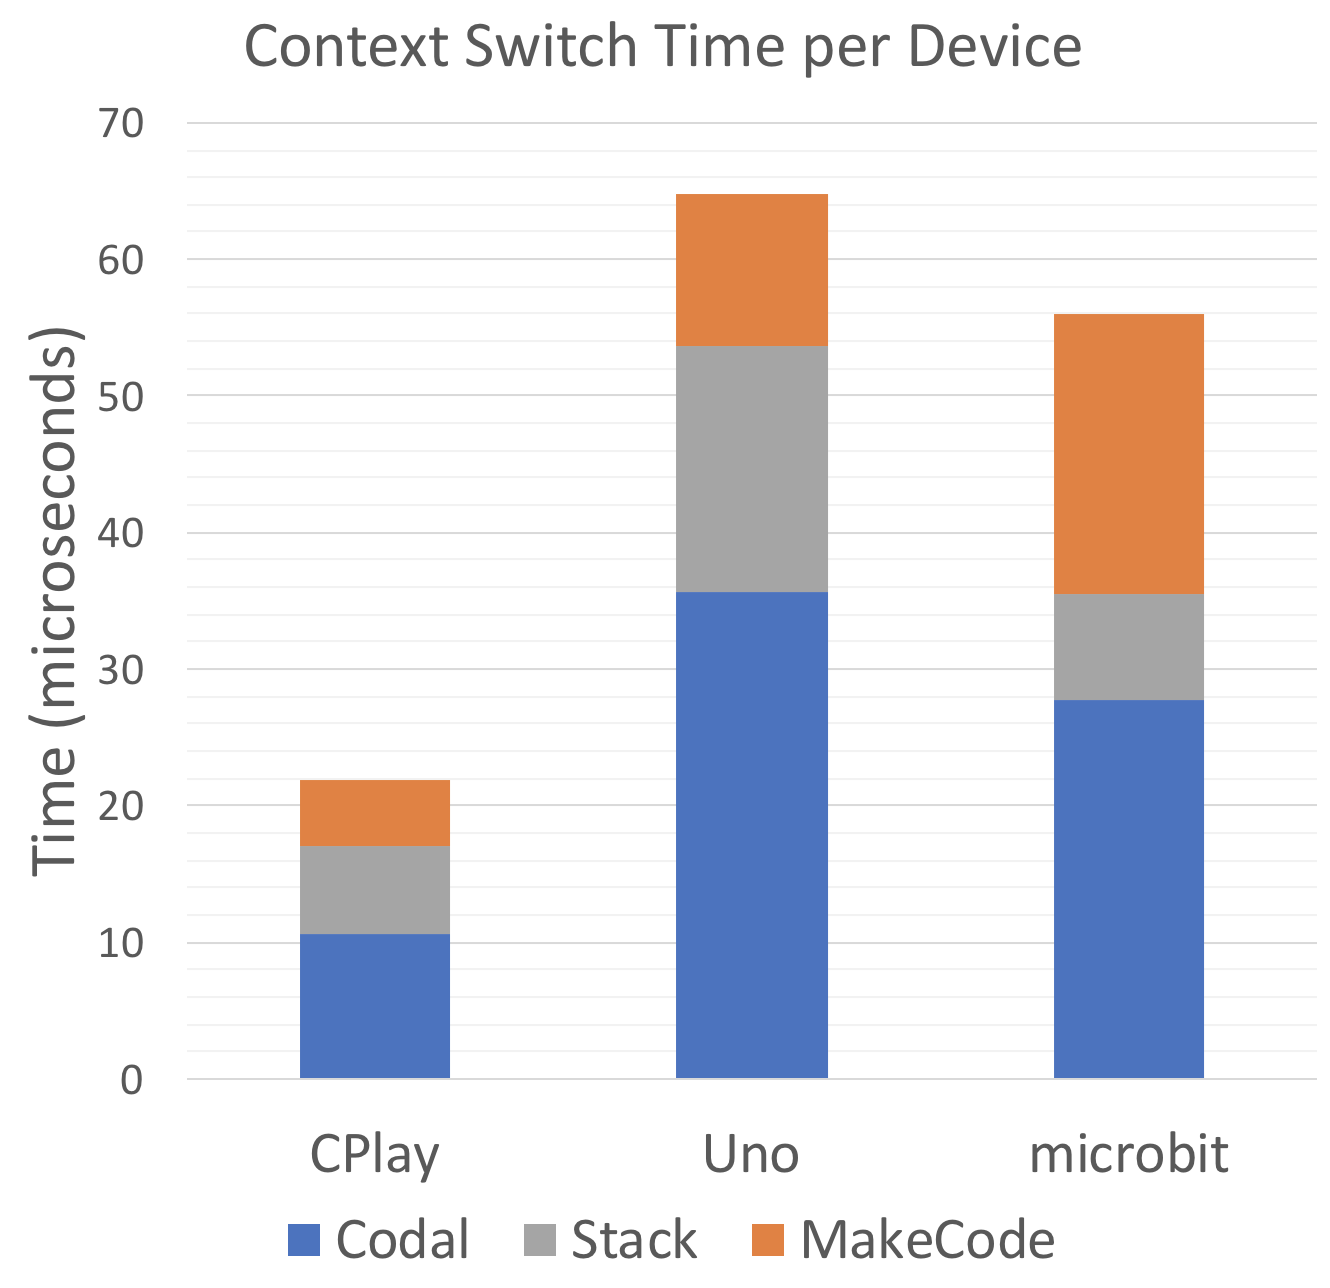
\includegraphics[width=.7\columnwidth]{images/context-switch.png}
\caption{\label{fig:context-switch}Base context switch profiles per device.}
\end{figure}

\begin{figure}[ht]
    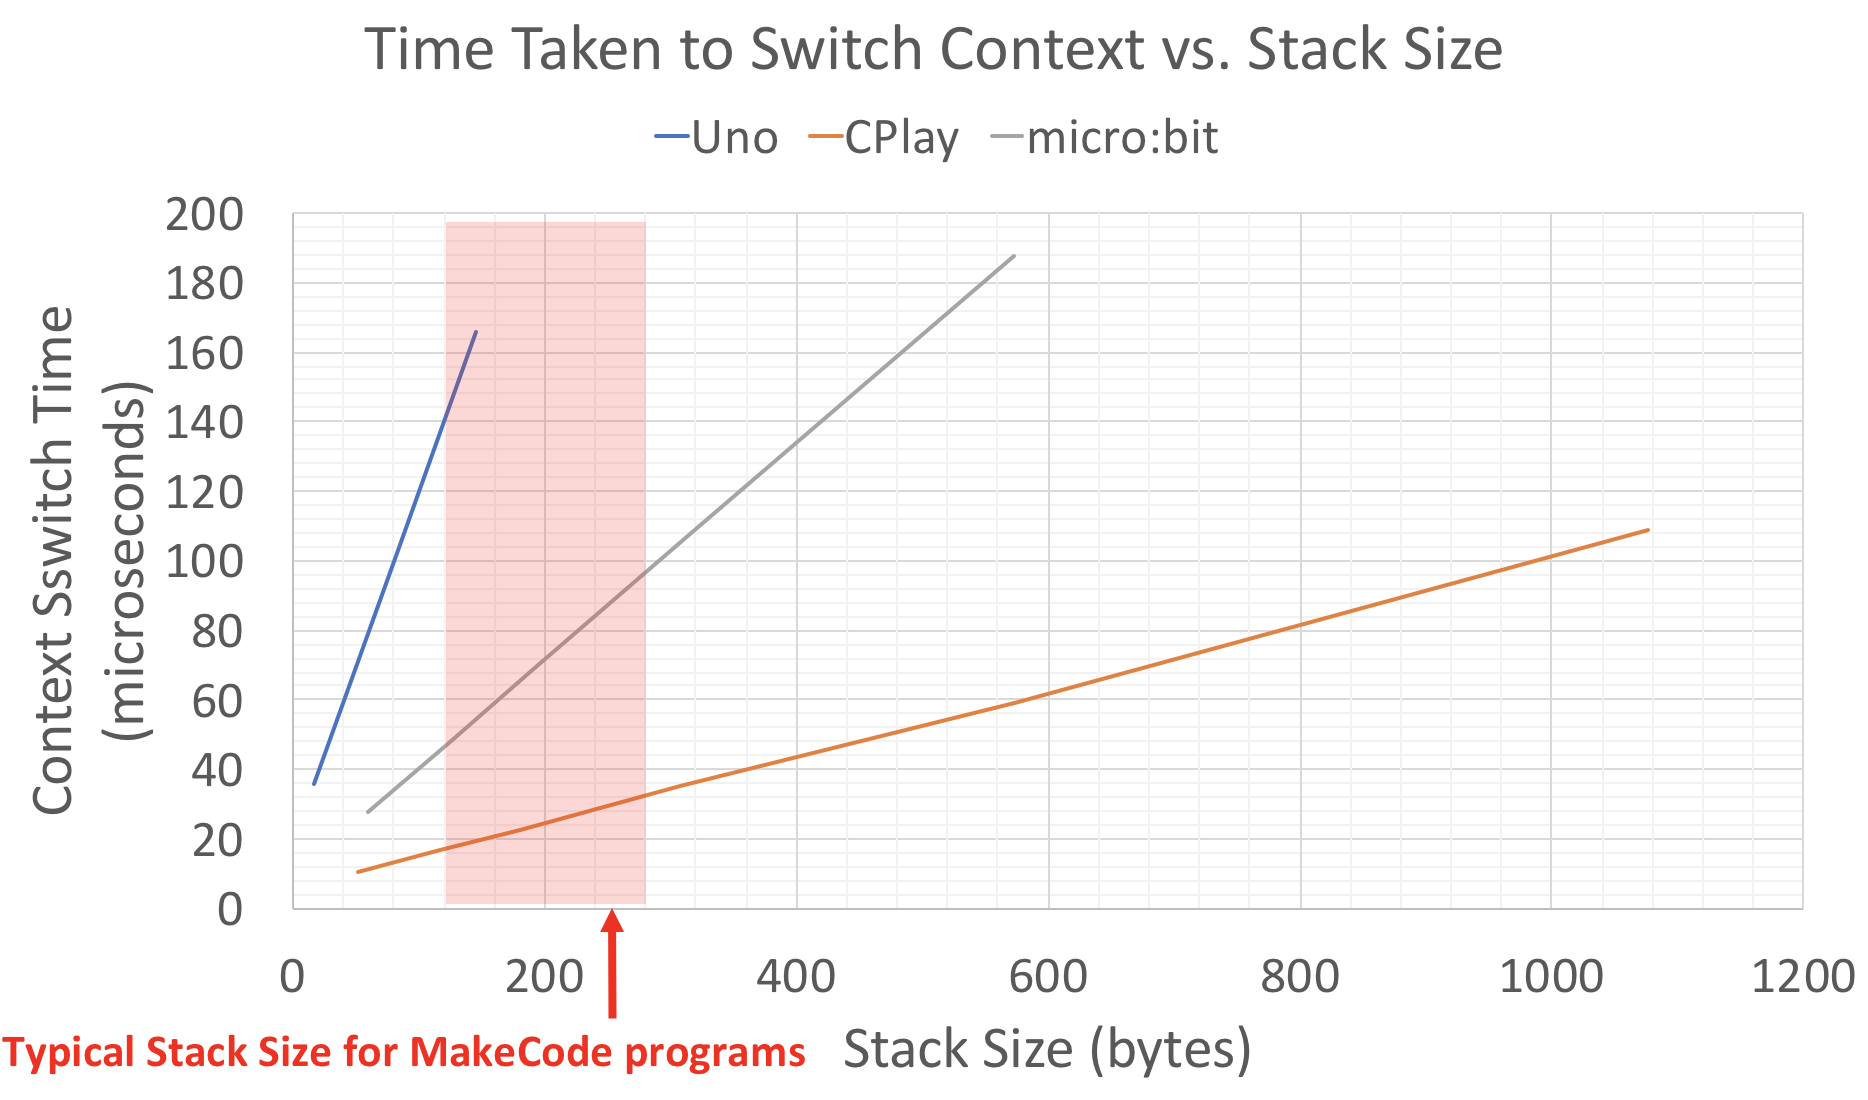
\includegraphics[width=.99\columnwidth]{images/context-vs-stack.png}
\caption{\label{fig:context-vs-stack}Time taken to perform a context switch against stack size.}
\end{figure}

To evaluate the performance of \CON's scheduler we conducted a test that created two fibers, continuously swapped context, and measured the time taken to complete the context switch.
We performed this test in both STS and C++ and the resulting profiles can be seen in Figure~\ref{fig:context-switch}, which
breaks the context switch down into three phases:
(1) \CON, the time it takes to perform a context switch in \CON;
(2) Stack, the time taken to page out the \MC stack; and
(3) \MCN, the overhead added by the \MC wrappers.

From these results, we observe that context switches generally take tens of microseconds. The cost of \CON's stack paging approach can also be a significant, but not dominant cost. The cost of stack paging would of course grow with stack depth. Figure~\ref{fig:context-vs-stack} therefore profiles the time a context switch takes with an increasing stack size across all three devices in \CON. This is similar to the previous test, except we placed bytes (in powers of 2) on the stack of each fiber, starting from 64 and finishing at 1024. The difference in gradients, and ranges of values can be put down to device capability. For instance, the Uno has an 8-bit word size, which means more instructions are required to copy the stack, therefore as the stack size increases, so does context switch time. The vertical band indicates typical stack sizes for \MC programs based on a representative set of examples.

%For the uno, the context switch profile is for the native implementation only.

\subsection{Performance of Asynchronous Operations}

% \begin{table}[h]
% \centering
% \begin{tabular}{c|c|c|}
%     \cline{2-3}
%                                                                                                                 & \begin{tabular}[c]{@{}c@{}}RAM Overhead\\ (bytes)\end{tabular} & \begin{tabular}[c]{@{}c@{}}Processing Overhead\\ (microseconds)\end{tabular} \\ \hline
%     \multicolumn{1}{|c|}{Create a Fiber}                                                                        & 136                                                            & 35.4                                                                         \\ \hline
%     \multicolumn{1}{|c|}{APC}              & 32                                                             & 4.01                                                                         \\ \hline
%     \multicolumn{1}{|c|}{APC with Sleep} & 204                                                            & 32.4                                                                         \\ \hline
%     \end{tabular}
% \caption{\label{table:time-ram-consumption}RAM consumption and processing time for various asynchronous operations in \CO.}
% \end{table}

To gauge the cost of asynchronous operations in \CON, we tested three commonly used code paths, designed to determine the efficiency of \CON's \emph{fork-on-block} Asynchronous Procedure Call (APC) mechanism that underpins all event handlers in \MC and \CON. We measured the RAM and processor cost of: (1) creating a fiber; (2) handling a non-blocking APC call; and (3) handling a blocking APC call. Again, the CPX was used for this experiment.

Non-blocking APC calls, the best case, have a small overhead of 32 bytes of RAM and 4.01 microseconds of processing time. Blocking APC calls, the worst case, incur a large overhead of 204 bytes of RAM and 32.4 microseconds of processor time. Simply creating a fiber costs 136 bytes of RAM and 35.4 microseconds of processing time. These results highlight the performance gains of the opportunistic fork-on-block mechanism over a naive approach that would execute every event handler in a separate fiber.

\subsection{Flash Memory Usage}

\begin{table}[h]
\centering
\begin{tabular}{c|c|c|c|}
\cline{2-4}
                                                                                                & CPX & micro:bit & Uno  \\ \hline
\multicolumn{1}{|c|}{\MC}                                                                       & 20.46 & 12.14     & 7.79 \\ \hline
\multicolumn{1}{|c|}{\CO}                                                                       & 29.85 & 34.35     & 13.7 \\ \hline
\multicolumn{1}{|c|}{\begin{tabular}[c]{@{}c@{}}Supporting Libraries\end{tabular}} & 14.99 & 24.28     & -    \\ \hline
\multicolumn{1}{|c|}{C++ Standard Library}                                                     & 43.14 & 24        & 1.03 \\ \hline
\end{tabular}

\caption{\label{table:flash-consumption}The total flash consumption of code required to support \MC (kB).}
\vspace{-20pt}
\end{table}

MCUs make use of internal non-volatile FLASH memory to store program code. Table~\ref{table:flash-consumption} shows the per device flash consumption of each software library used in the final \MC binary. To obtain these numbers, we profiled the final map file produced after compilation. The ordering of the table aligns with the composition of the software layer: \MC builds on \CO which builds on the C++ standard library and supporting libraries.
In comparison to other languages, \MC and \CO consume a small amount of flash: CircuitPython consumes 201.404 kB, micropython consumes 228.044 kB, and Espruino consumes 142.196 kB of flash. This means that users can write applications in \MCN, without the worry of running out of flash memory.

From the bottom up, the profile of the standard library changes dramatically for each device: The Uno has a very lightweight standard library; the microbit uses 64-bit integer operations (for timers) which requires extra standard library functions; and the CPX requires software floating point operations pulling in more standard library functions.

The size of \CO and \MC scales linearly with the amount of functionality a device has, due to the component oriented nature of \CO and transitively \MCN. For instance the Uno has few onboard components when compared to the CPX and micro:bit. The modular composition of \CO allows us to support multiple devices with a variety of feature sets, while maintaining the same API at the \MC layer.

\subsection{RAM Memory Usage}

\begin{table}[h]
\centering
\begin{tabular}{c|c|c|c|}
\cline{2-4}
                                                                                                & CPX & micro:bit & Uno   \\ \hline
\multicolumn{1}{|c|}{\MC}                                                                       & 0.612 & 1.069     & 0.074 \\ \hline
\multicolumn{1}{|c|}{\CO}                                                                       & 0.369 & 0.214     & 0.156 \\ \hline
\multicolumn{1}{|c|}{\begin{tabular}[c]{@{}c@{}}Supporting Libraries\end{tabular}} & 0.312 & 0.923     & -     \\ \hline
\multicolumn{1}{|c|}{C++ Standard Library}                                                     & 0.161 & 0.149     & 0.074 \\ \hline
\end{tabular}
\caption{\label{table:ram-consumption}The total static RAM consumption for an \MC binary (kB).}
\vspace{-20pt}
\end{table}

Table~\ref{table:ram-consumption} shows the per device RAM consumption of each software library used in the final \MC binary. To obtain these numbers, we profiled the final map file produced after compilation. At runtime \MC also dynamically allocates additional memory: 1.56 kB for the CPX, 560 bytes for the micro:bit, and 644 bytes for the Uno. We can also see that in all cases, the RAM consumption of \MC and \CO is well within the RAM available of each device.

\MC and \CO consume a small amount of resources in comparison: CircuitPython (a derivative of micropython) consumes 12,802 kB, micropython consumes 9.472 kB, and Espruino consumes 5.270 kB of RAM. On the microbit the Bluetooth stack requires 8kB of RAM to run, due to micropython's RAM consumption this means that Bluetooth is inoperable. Comparatively, Espruino does enable the Bluetooth stack, but due to the overhead incurred, users have \textasciitilde300 bytes available for their programs.

% Add globals maps and profile of listener and fiber.

% The CPX runtime is the largest, as the CPX device has lots of on-board
% components, and this runtime shares much of its code with other SAMD21 \MC targets.
% The compiled C++ runtime is 114k in total, with \CO accounting for 29k, with an
% additional 15k from libmbed. The \MCN-common-packages adds 20k, and also in
% an additional 49k of math support libraries (floating point operations,
% including trigonometry and number printing/parsing).
% As the SAMD21 has 256k of flash, we did not worry about optimizing this runtime for space.

% On the Uno, which has 32k of flash, the much \MC runtime is 8k and \CO is 14k (since
% the Uno only requires basic GPIO, i2c and serial drivers), leaving 10k for user code.

% The TypeScript part of the runtime is 1060 statements on the CPX and 216 on the Uno.
% In our microbenchmarks, 99\% of that runtime is tree-shaken away.

\subsection{Compiling Static TypeScript}

When compiling, the entire STS program, including the runtime, is passed to the TypeScript (TS) language service for parsing. Then, only the remaining part of the program (after code shaking) is compiled to native code. On a modern laptop, using Node.js, TS parsing and analysis takes about 0.1 ms per statement, and \MC compilation to native code takes about 1 ms per statement.
While the TS compiler has been optimized for speed, \MCN's native compilation process has not been. For example, the CPX TS pass is dominated by compilation of the device runtime and takes about 100ms, whereas the \MC pass typically only includes a small user program and a small bit of the runtime, resulting in less than 100ms. Thus, typical compilation times are under 200 ms for typical user programs of 100 lines or less.

\subsection{Extensibility}

Creating a device in \CO is trivial once a processor has been ported. The porting of a processor is where we observe the largest overhead, as low-level implementation of drivers for I2C, Serial, and SPI have to be re-written. Due to \CON's abstraction model, once low-level drivers have been implemented, drivers for higher level components like Accelerometers, which depend on high-level interfaces for low-level drivers, can be immediately adopted if hardware is present. A similar technique is used in \MC for simulators.

% Not really a result, more of a description of design, with an anecdotal comment about speed.

% should be moved further up and described alongside AVR VM vs. Native

% The AVR VM was specifically designed for high code density, since \CO
% leaves less than 10k for TS runtime and user code on the Uno. The interpreter is implemented in assembly, always included with the program, and is around 0.5k.
% There are about 30 opcodes, some of which can take 1 or 2 byte arguments. There are also a few combined opcodes, representing a sequence of one argument-less opcode, and one with an argument, which improves code density by about 25\%. Opcodes are direct offsets into the code of the interpreter, speeding up execution. They operate on a stack (mainly for function calls) and a special scratch register. There is essentially no stack space overhead compared to native AVR compilation. The speed overhead is around 4x-5x (with respect to native) for computational tasks.


%\subsection{Implementation}
% •	\CO (SAMD21 and AVR): base runtime (C++ only)
% •	pxt
% •	pxt-common-packages: C++ and Static TypeScript
% •	pxt-adafruit
% •	pxt-arduino-uno
% •	pxt-monaco, pxt-blockly

%mmoskal [10:10 AM]
%`pxt checkdocs --snippets --re perf --stats`
% [10:11]
% I compile empty sample first twice, to reduce JIT costs
% [10:12]
% also, the first "compile prep" is slightly more costly, since it parses a hex file

\section{Related Work}
\label{sec:related}
%% potentially cut this
\subsection{Novice programming environments}

Arduino~\cite{buildingArduino2014} is an environment for programming microcontrollers, aimed at novices. However, its C++-based APIs introduces barriers for novice programmers~\cite{blikstein2013gears}. Scratch~\cite{ScratchCACM2009} is a widely adopted, event-based visual programming environment designed to introduce novice programmers to computer science concepts. Extensions enable the programming of physical devices with Scratch. However, devices require constant tethered connections to operate, restricting potential projects~\cite{dougherty2012maker}. ArduBlock~\cite{Ardubloc28:online} brings visual programming to the Arduino but it lacks the event-based blocks Scratch users are familiar with.

With the environments above, additional software must be installed, which creates barriers for novice users in restrictive environments. MakeCode and CODAL require \emph{no installation} to support a diverse user base and support \emph{event-based higher-level languages} to help beginners get a head start in the world of the microcontroller.

\subsection{Virtual machine-based languages}

Recently, virtual machines supporting most of the semantics of higher level languages like JavaScript, Java, and Python, have been ported to 32-bit microcontrollers by maker communities.~\cite{dougherty2012maker} Examples include: MicroPython~\cite{MicroPython}, CircuitPython, and Espruino~\cite{espruinoBook}. These VMs consume a large amount of RAM and flash memory and run significantly slower than native languages.

The research community has worked to bring higher level languages to microcontrollers~\cite{koshy2005vmstar,st2009picobit,vaugon2015programming}. Rather than running a full-featured VM, others enable higher level languages to run efficiently by stripping out advanced language features, in favor of efficient, native execution~\cite{varma2004java}. Comparing these solutions to our solution is challenging due to a misalignment in evaluation metrics and microcontrollers. For example, the PICOBit uses an 8-bit MCU, and evaluates the cost of a VM, without the cost of a runtime environment. Simply accounting for a 32-bit MCU in this case, results in factor of 4 multiplication of most metrics.

Our approach bears most similarity to~\cite{varma2004java}, where we compile higher level languages to an \emph{optimized, event-driven} C++ runtime (\CON).

\subsection{Embedded runtime environments}

%Embedded runtime environments can range from simple C++ classes that control hardware, to real-time operating systems (RTOSs) with scheduling and memory management.

Arduino~\cite{buildingArduino2014} is an example of a simple platform where the developer uses high-level APIs to control hardware; there is no scheduler and memory management is discouraged, with a heavy emphasis on 
the use of global variables.

TinyOS~\cite{levis2005tinyos}, Contiki~\cite{dunkels2012contiki}, RIOT OS~\cite{baccelli2013riot}, Mynewt~\cite{ApacheMy53:online} mbed OS~\cite{ARMmbed}, Zephyr~\cite{HomeZeph63:online} are RTOS solutions known widely in the systems community. The majority focus on the networking features of sensor based devices and commonly adopt a preemptive scheduling model, which leads to competition over resources resolved using locks and condition synchronization primitives. Contiki has a cooperative scheduler but uses proto-threads to store thread context --- local variables are not allowed as the context of the stack is not stored.

Although the platforms above are widely used by C/C++ developers, none of these existing solutions align well with the programming paradigms seen in higher level languages. \CO \emph{bridges that semantic gap between the higher level language and the microcontroller}, offering appropriate abstractions and higher level primitives written natively in C++.

\subsection{Flashing microcontrollers}

There are two common ways to transfer a program to the flash of a microcontroller: for embedded developers, a specialized debugger chip; for hobbyists, a custom serial protocol~\cite{AVRDUDEA15:online}. Both approaches require operating system drivers. ARM's mbed platform provides DAPLink~\cite{GitHubAR5:online}, firmware that presents itself to an external computer as a USB pen drive. DAPLink exposes a virtual file system that caters for normal file system behavior and handles the decoding of Intel HEX files~\cite{IntelHEX} --- the firmware consumes 66 kB of flash and 13 kB RAM. \UF contributes a new file format that \emph{greatly simplifies} the virtual file system approach, reducing complexity of the firmware and code size.

% talk about old protocols for flashing protocols, talk about mbed, talk about UF2

% % * programming languages for microcontrollers
% %     - discuss low level languages
% %     - talk about approaches to higher level languages by communities
% %     - talk about approaches to higher level languages by research
% %     - contextualise against our approach
% \subsection{Programming languages for novice users}


% Java-through-C compilation: \cite{varma2004java}

% VMSTAR: synthesizing scalable runtime environments for sensor networks \cite{koshy2005vmstar}

% % * Embedded Runtime Environments
% %     -largely remains as is.
% \subsection{Embedded Runtime Environments}

% Typically written in C and/or C++, environments for MCU programming all share a common design goal: to support developers by providing primitives and programming abstractions. Platforms can range from simple C++ classes that control hardware, to real-time operating systems (RTOSs) with scheduling and memory management.

% Arduino~\cite{buildingArduino2014} is an example of a simple platform where the developer uses high-level APIs to control hardware; there is no scheduler, and memory management is discouraged through a heavy emphasis on global variables.

% TinyOS~\cite{levis2005tinyos}, Contiki~\cite{dunkels2012contiki}, RIOT OS~\cite{baccelli2013riot}, Mynewt~\cite{ApacheMy53:online} mbed OS~\cite{ARMmbed}, Zephyr~\cite{HomeZeph63:online} are RTOS solutions known widely in the embedded systems community. The majority focus on the networking features of sensor based devices and commonly adopt a preemptive scheduling model, which leads to competition over resources resolved using locks and condition synchronization primitives. Contiki has a cooperative scheduler, but uses proto-threads to store thread context --- local variables are not allowed as the context of the stack is not stored.

% Although the platforms above are widely used by C/C++ developers, none of these existing solutions align well with the programming paradigms seen in higher level languages. \CO bridges that semantic gap between the higher level language and the microcontroller, offering appropriate abstractions and higher level primitives written natively in C++.


% \subsection{Programming microcontrollers}

% \paragraph{Tethering a device} Scratch's device extensions~\cite{ScratchCACM2009} and Arduino's Firmata library~\cite{Firmata} take the tethered approach. However, in the educational and maker~\cite{dougherty2012maker} settings, MCUs often are embedded in projects. Here, this method has limited utility, as in such projects the MCU is powered by battery and is not connected to a host.

% \paragraph{Loading a pre-compiled native binary onto a device}
% Arduino~\cite{buildingArduino2014}, mbed~\cite{ARMmbed}, and other C-based solutions require installation of additional software and knowledge of low-level languages. These requirements do not suit a diverse demographic of inexperienced users.

% \paragraph{Interpretting pre-compiled bytecode on the device}
% Java for embedded systems~\cite{ClausenTOPLAS}

% suffer in terms of performance on small MCUs, operating slower than native C++ code, and consuming most of the resources (flash and RAM) of the MCU.

% \paragraph{Loading a compiler and virtual machine onto a device}
% MicroPython~\cite{MicroPython} and Espruino~\cite{espruinoBook};

% Our platform slots into options 2 and 3, using the \MC architecture and USB pen drives to avoid the need for installation of native applications or device drivers. Our use of STS provides better performance than the MicroPython and Espruino solution, as demonstrated in the evaluation,
% and allows us to fit in the very constrained space of the Uno.




% \subsection{Programming microcontrollers}

% talk about old protocols for flashing protocols, talk about mbed, talk about UF2

\section{Conclusion}
\label{sec:conclude}

We have presented \MCN, a \emph{no installation}, web-based programming environment, that supports novice programmers with \emph{block-based and text-based higher-level languages}, and compiles programs \emph{in the browser}. So as to not compromise the spatial efficiency of the microcontroller, we created \CON, a C++ runtime that \emph{bridges the semantic gap} between higher level languages in \MC and C++. To transfer programs compiled by \MC to the microcontroller without the installation of any drivers, we created \UFN, a new bootloader and file format that enables the \emph{simplified}, \emph{driverless} programming of microcontrollers.

Combined, our approach to running higher level languages on microcontrollers is up to 50x more performant versus other approaches. Further, by using modern tooling, and higher level languages, our approach lowers the barrier to entry for microcontroller programming.

% We have presented and evaluated a new platform designed to bring modern language features and tooling to microcontrollers. Our aim was to do this in an extensible way which supports novice programmers with block-based programming while providing a progression path to a text-based scripting language and ultimately to C++. Our platform includes a new C++ runtime called \CO which is designed to make efficient use of the limited resources on a microcontroller. A statically-typed subset of TypeScript forms the basis for both blocks- and text-based programs, created and compiled using a new web-based IDE named \MC.

% Our aspiration is to enable a new paradigm for programming pretty-much anything, even an Arduino Uno-class MCU, by anyone -- novices and professional developers alike, from anywhere, i.e. without the need for traditional heavyweight embedded toolchains and IDEs. Our open-source implementation is in daily use, with thousands of users writing programs targeted at several different MCU-based devices. In this sense, we have achieved our goal. We also have anecdotal evidence that our platform -- in terms of both language and tooling -- is intuitive to professional developers with no experience of embedded development.


\section*{Acknowledgements}

The authors would like to thank the members of the MakeCode team for their many contributions to the success of the platform: Abhijith Chatra, Sam El-Husseini, Caitlin Hennessy, Guillaume Jenkins, Richard Knoll, Galen Nickel, Jacqueline Russell, and Kesavan Shanmugam.

%% Bibliography
\bibliography{paper}

\appendix
\pagebreak
\section{Static TypeScript Subtype Relation}


In STS, $S$ is a subtype of a type $T$ if one of the following is true:
\begin{itemize}
\item $S$ and $T$ are identical types;
\item $S$ is the Undefined type;
\item $S$ is the Null type and $T$ is not the Undefined type;
\item $S$ is an enum type and $T$ is the primitive type Number;
\item $S$ is a string literal type and $T$ is the primitive type String;
\item $S$ and $T$ are class types and all the following are true:
\begin{itemize}
  \item $S$ is derived from $T$ (via \emph{extends} clauses);
  \item checkProps($S$,$T$) holds;
\end{itemize}
\item $S$ is a class/record type and $T$ is a record type and
\begin{itemize}
  \item checkProps($S$,$T$) holds;
\end{itemize}
\item $S$ and $T$ are function types such that all the following hold:
\begin{itemize}
  \item $S$ has at least as many parameters as $T$;
  \item each parameter type in $T$ is a subtype of the corresponding parameter type in $S$;
  \item the result type of $T$ is Void, or the result type of $S$ is a subtype of that of $T$;
\end{itemize}
\item $S$ and $T$ are array types and all the following hold:
\begin{itemize}
\item $T$ has a numeric index signature with element type $U$,
    and $S$ has a numeric index signature with element type $V$
    such that $V$ is a subtype of $U$;
\item checkProps($S$,$T$) holds.
\end{itemize}
\end{itemize}

Given types $S$ and $T$, checkProps($S$,$T$) holds if for each property $N$ in $T$,
$S$ has a property $M$ where all of the following are true:
\begin{itemize}
\item $M$ and $N$ have the same name;
\item the type of $M$ is a subtype of the type of $N$;
\item $M$ and $N$ are both public, or $M$ and $N$ are both
      private (protected) and originate in the same declaration,
      or $N$ is protected and $S$ is a class derived from class $T$
\end{itemize}

\section{Artifact appendix}

Submission and reviewing guidelines and methodology: \\
{\em http://cTuning.org/ae/submission.html}

%%%%%%%%%%%%%%%%%%%%%%%%%%%%%%%%%%%%%%%%%%%%%%%%%%%%%%%%%%%%%%%%%%%%%
\subsection{Abstract}

This artifact allows others to reproduce the results seen in this paper for MakeCode and Codal, using the BBC micro:bit. The artifact contains an offline build environment for codal and MakeCode, allowing evaluators to test and build programs locally. In addition, we also provide espruino and micropython virtual machines to further increase repeatability of our results. Evaluators should download the virtual machine containing all pre-requisite tools, and use an oscilloscope to observe wave forms (used for timing) generated by the micro:bit, and a serial terminal to observe results reported from the micro:bit over serial.


\subsection{Artifact check-list (meta-information)}

{\small
\begin{itemize}
  \item {\bf Program:} MakeCode \& Codal
  \item {\bf Compilation:} arm-none-eabi-gcc
  \item {\bf Binary:} espruino, and micropython binaries included; others compiled during testing
  \item {\bf Run-time environment:} Codal
  \item {\bf Hardware:} BBC micro:bit
  \item {\bf Output:} Waveforms, and serial output
  \item {\bf Publicly available?:} Yes
  \item {\bf Artifacts publicly available?:} Yes
  \item {\bf Artifacts functional?:} Yes
  \item {\bf Artifacts reusable?:} Yes
  \item {\bf Results validated?:} Yes
\end{itemize}

%%%%%%%%%%%%%%%%%%%%%%%%%%%%%%%%%%%%%%%%%%%%%%%%%%%%%%%%%%%%%%%%%%%%%
\subsection{Description}

\subsubsection{How delivered}

The artifact is available on GitHub:\\[5pt]\url{https://lancaster-university.github.io/lctes-artefact-evaluation/}\\[5pt] And a virtual machine, based on debian, containing all the required software to reproduce our results is available here:\\[5pt]\url{https://drive.google.com/open?id=1nxiorz6NRqjen89G59RCOEMklqAyaUv7}

\subsubsection{Hardware dependencies}

\begin{itemize}
    \item A BBC micro:bit
    \item An oscilloscope
    \item A computer capable of running a virtual machine
\end{itemize}

\subsubsection{Software dependencies}

\begin{itemize}
    \item A virtual machine obtained from the URL above.
    \item A serial terminal.

\end{itemize}

%%%%%%%%%%%%%%%%%%%%%%%%%%%%%%%%%%%%%%%%%%%%%%%%%%%%%%%%%%%%%%%%%%%%%
\subsection{Installation}

Use virtual box to install the image located at:\\[5pt]\url{https://drive.google.com/open?id=1nxiorz6NRqjen89G59RCOEMklqAyaUv7}\\[5pt]
and the VirtualBox extension pack:\\[5pt]\url{https://www.virtualbox.org/wiki/Downloads}
%%%%%%%%%%%%%%%%%%%%%%%%%%%%%%%%%%%%%%%%%%%%%%%%%%%%%%%%%%%%%%%%%%%%%
\subsection{Experiment workflow}

Tests generally follow the following sequence of steps:

\begin{enumerate}
    \item Perform small program modifications.
    \item Compile the program.
    \item Transfer program to the micro:bit (flashing).
    \item Observe either a waveform generated by the micro:bit using an oscilloscope, or serial output from the micro:bit using a serial program.
\end{enumerate}

%%%%%%%%%%%%%%%%%%%%%%%%%%%%%%%%%%%%%%%%%%%%%%%%%%%%%%%%%%%%%%%%%%%%%
\subsection{Evaluation and expected result}

We expect the results to be the same as those reported in the paper. The observed waveforms may differ in time due to different compilers, oscilloscopes, and oscilloscope calibration.

%%%%%%%%%%%%%%%%%%%%%%%%%%%%%%%%%%%%%%%%%%%%%%%%%%%%%%%%%%%%%%%%%%%%%
\subsection{Experiment customization}

All tests provided have a clear set of corresponding instructions that evaluators should follow to observe the same results. Any steps involving customisation have been minimised.

%%%%%%%%%%%%%%%%%%%%%%%%%%%%%%%%%%%%%%%%%%%%%%%%%%%%%%%%%%%%%%%%%%%%%
\subsection{Notes}

The virtual machine contains a folder named `evaluators' which is placed in the home directory of the lctes user. The username for the virtual machine is: \textit{lctes} and the password is: \textit{lctes2018}. To become super user, type \textit{su} in a terminal, and enter the same password (\textit{lctes2018}).

Once logged in, and in the `evaluators' directory, you can view the tests as markdown files in the `docs' directory. Alternately, these markdown documents can also be viewed on the web by running `mkdocs serve' in the evaluators folder, or browsing to:\\[5pt]\url{https://lancaster-university.github.io/lctes-artefact-evaluation/}\\[5pt] Which is a pre-built, and hosted version produced from the same source.

We recommend that you add the micro:bit usb device using the machine settings tab in virtual box as shown in the image below:\\

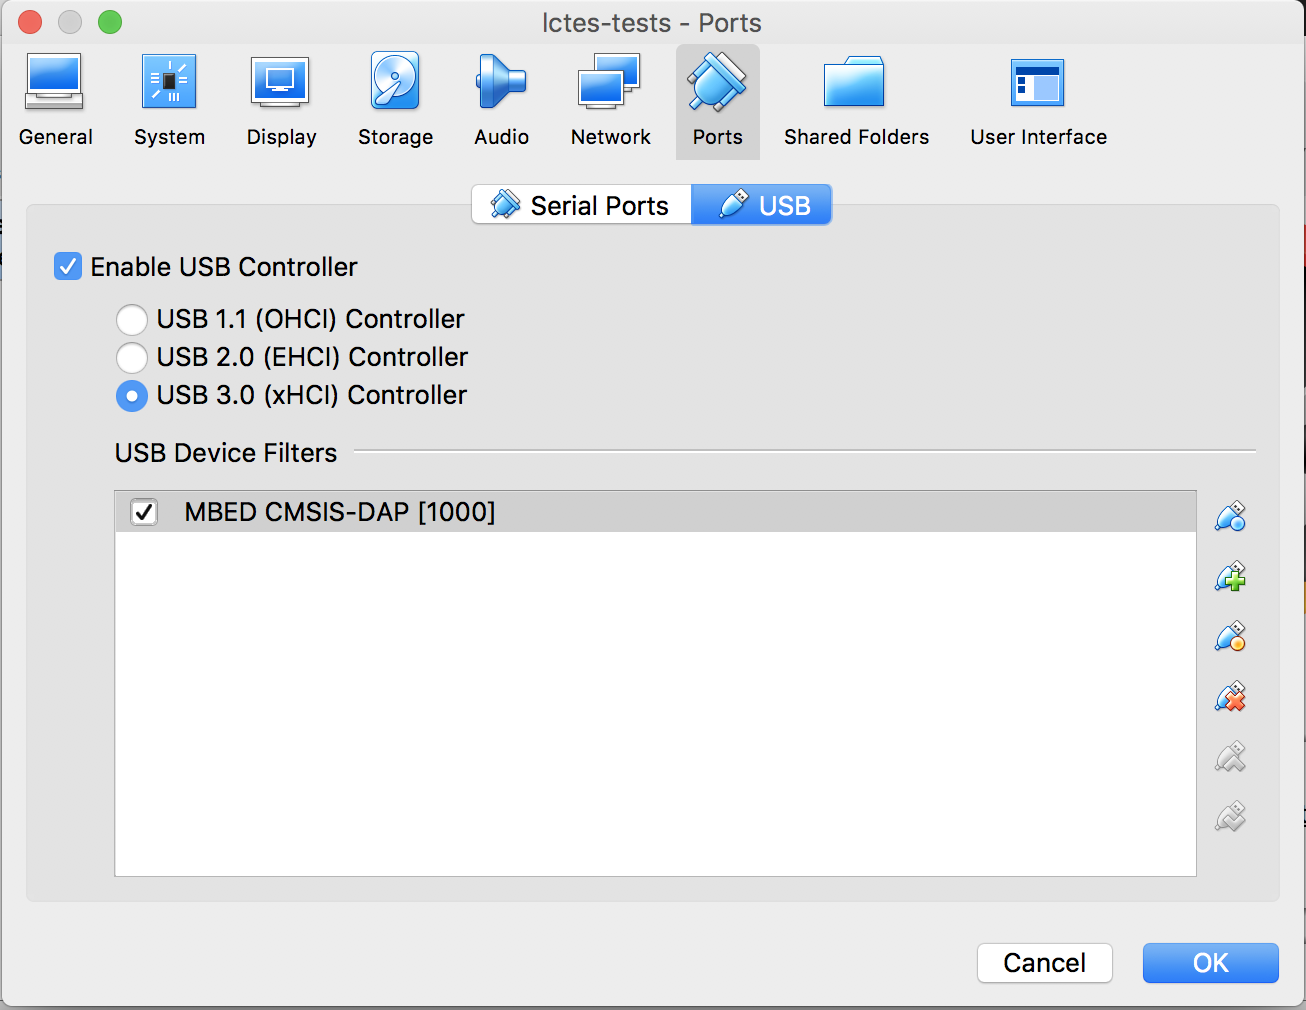
\includegraphics[width=\columnwidth]{images/virtualbox.png}

We also have a convenience script for mounting a shared folder between the host and the vm. Simply create a shared folder named `lctes-vm-dir' and run `sh mount.sh' (contained in evaluators) as a super user to mount the shared folder to vb-share (also contained in evaluators). Shared folder creation in VirtualBox is pictured below:\\

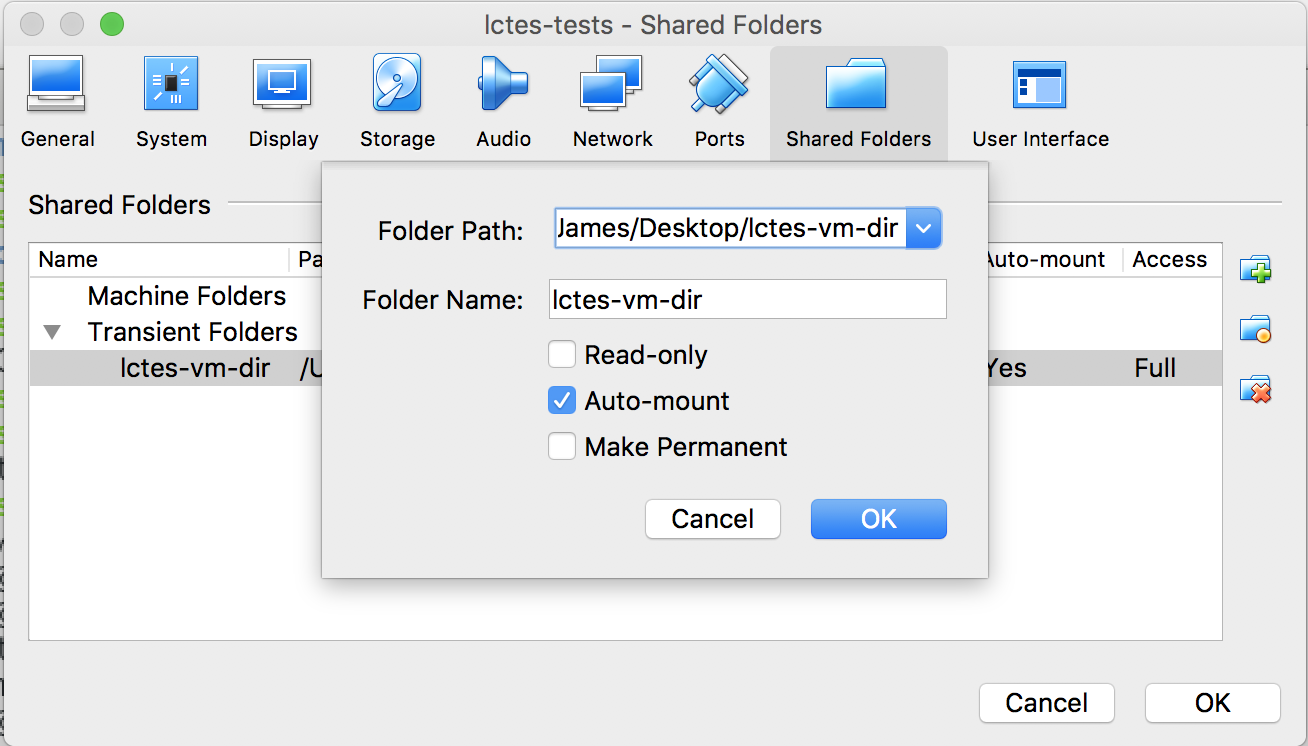
\includegraphics[width=\columnwidth]{images/shared-folder.png}

\end{document}
